% libraries
\usetikzlibrary{positioning}

% styles
\tikzstyle{module} = [draw, fill=blue!10, text centered, rounded corners, minimum height=1cm, minimum width=2.5cm]
\tikzstyle{file} = [module, fill=red!10]

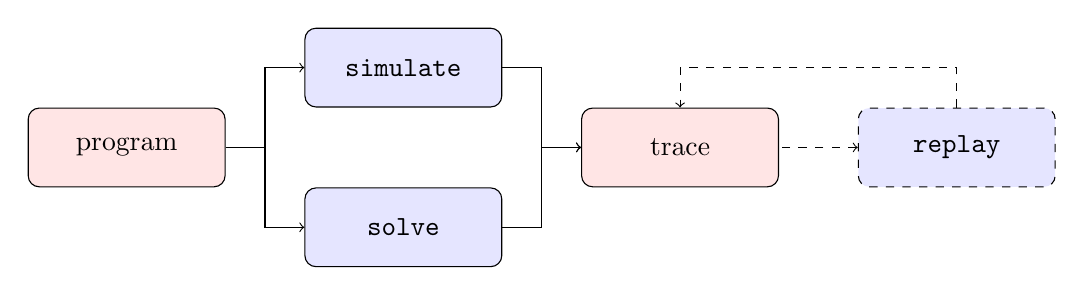
\begin{tikzpicture}[auto]

  \node [file] (program) {program};

  \node [module] (simulate) [above right=0cm and 1cm of program] {\texttt{simulate}};
  \path [draw, ->] (program.east) -- ++(0.5, 0) |- (simulate);

  \node [module] (solve) [below right=0cm and 1cm of program] {\texttt{solve}};
  \path [draw, ->] (program.east) -- ++(0.5, 0) |- (solve);

  \node [file] (trace) [below right=0cm and 1cm of simulate] {trace};
  \path [draw, ->] (simulate.east) -- ++(0.5, 0) |- (trace);
  \path [draw, ->] (solve.east) -- ++(0.5, 0) |- (trace);

  \node [module, dashed] (replay) [right= of trace] {\texttt{replay}} edge [<-, dashed] (trace);
  \path [draw, dashed, ->] (replay) -- (replay.north |- simulate) -| (trace.north);

\end{tikzpicture}
